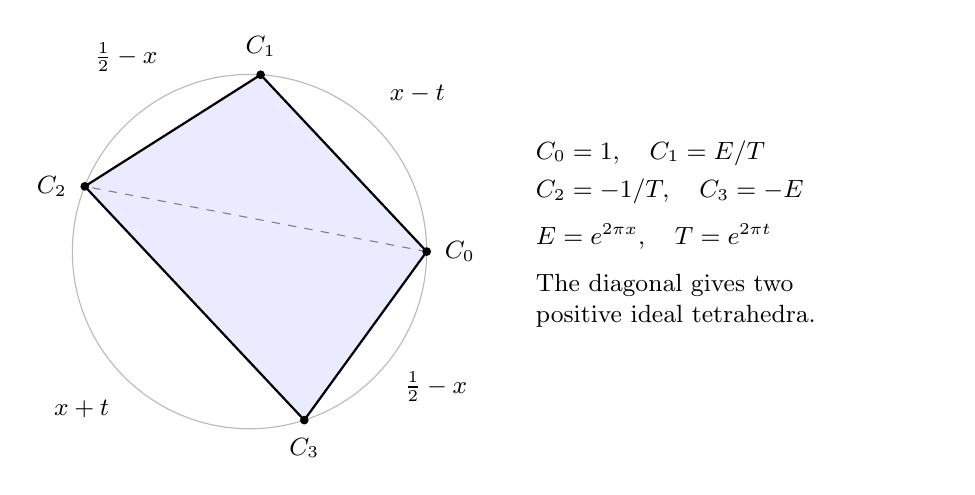
\begin{tikzpicture}[scale=2.25,every node/.style={font=\small}]
\coordinate(c0) at (1,0);
\coordinate(c1) at ({cos(86.4)},{sin(86.4)});
\coordinate(c2) at ({cos(158.4)},{sin(158.4)});
\coordinate(c3) at ({cos(288)},{sin(288)});
\draw[gray!55] (0,0) circle(1);
\fill[blue!8] (c0)--(c1)--(c2)--(c3)--cycle;
\draw[thick] (c0)--(c1)--(c2)--(c3)--cycle;
\draw[dashed,gray] (c0)--(c2);
\foreach \p/\lab/\pos in {c0/C_0/right,c1/C_1/above,c2/C_2/left,c3/C_3/below}
 {\fill(\p) circle(.7pt);\node[\pos=3pt] at(\p){$\lab$};}
\node at ({1.3*cos(43.2)},{1.3*sin(43.2)}) {$x-t$};
\node at ({1.3*cos(122.4)},{1.3*sin(122.4)}) {$\frac12-x$};
\node at ({1.3*cos(223.2)},{1.3*sin(223.2)}) {$x+t$};
\node at ({1.3*cos(324)},{1.3*sin(324)}) {$\frac12-x$};
\node[align=left,text width=5.1cm] at (2.75,.1)
 {$C_0=1,\quad C_1=E/T$\\[3pt]
  $C_2=-1/T,\quad C_3=-E$\\[6pt]
  $E=e^{2\pi\ii x},\quad T=e^{2\pi\ii t}$\\[6pt]
  The diagonal gives two\\positive ideal tetrahedra.};
\end{tikzpicture}
